\section{Additional Descriptives \& Diagnostics}\label{app:add_graphs_diags}


% \subsection{Word Count \& Verbosity Bias}\label{app:verbosity_diagnostics}

% \begin{figure}[h]
%     \centering
%     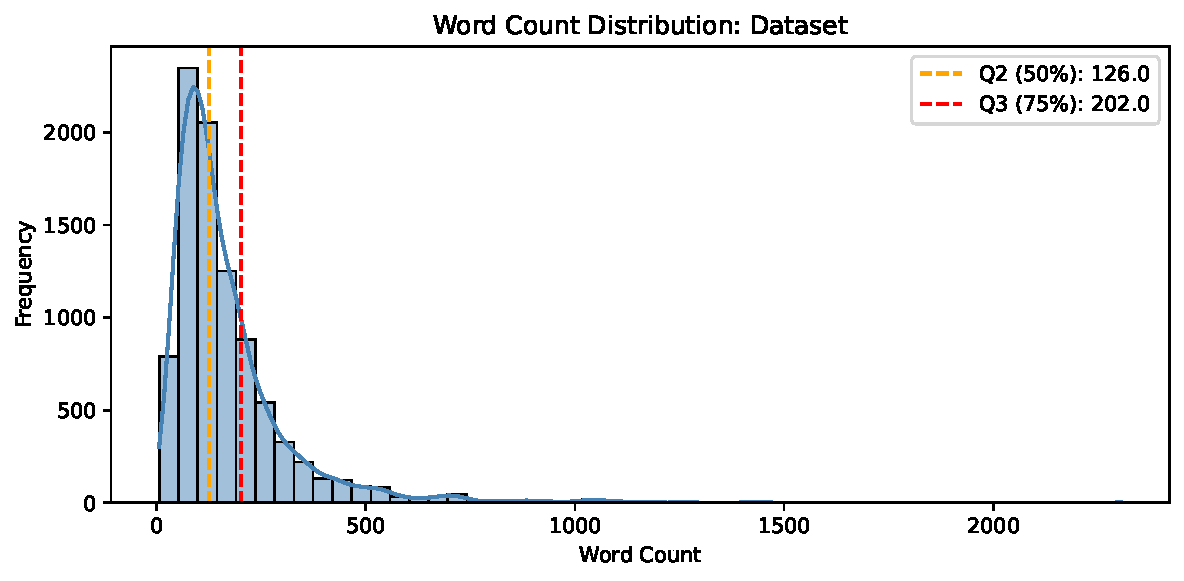
\includegraphics[width=0.8\textwidth]{figures/feedbackqa_word_count.pdf}
%     \caption{Empirical distribution of combined word counts (Question + Answer) for the FeedbackQA dataset. The dashed lines indicate the median ($Q(0.50) = 126$) and the 75th percentile ($Q(0.75) = 202$), which serve as the boundaries for the mature text brackets ($D_{Q3}$ and $D_{Q4}$) used in the verbosity bias assessment.}
%     \label{fig:feedbackqa_word_count}
% \end{figure}

% \begin{figure}[h]
%     \centering
%     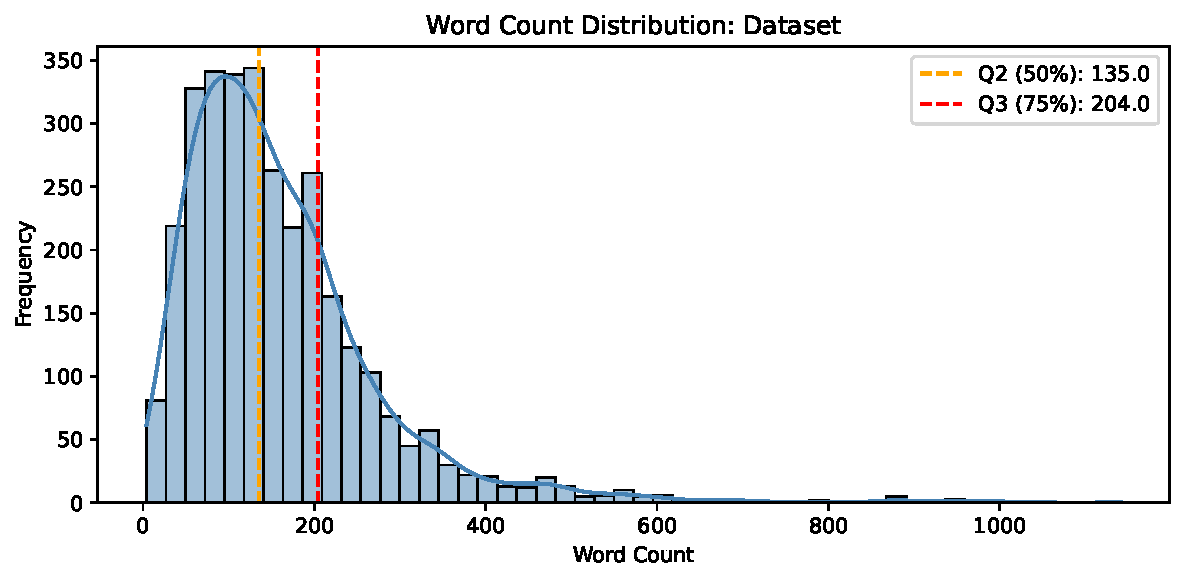
\includegraphics[width=0.8\textwidth]{figures/barter_word_count.pdf}
%     \caption{Empirical distribution of combined word counts (Title + Body + Requirements) for the Barter Deals dataset. The dashed lines indicate the median ($Q(0.50) = 135$) and the 75th percentile ($Q(0.75) = 204$), which serve as the boundaries for the mature text brackets ($D_{Q3}$ and $D_{Q4}$) used in the verbosity bias assessment.}
%     \label{fig:barter_word_count}
% \end{figure}


\subsection{Text-Length Descriptives and Residual Verbosity Sensitivity}
\label{app:verbosity_diagnostics}

\begin{figure}[htbp]
    \centering

    \begin{subfigure}{0.82\textwidth}
        \centering
        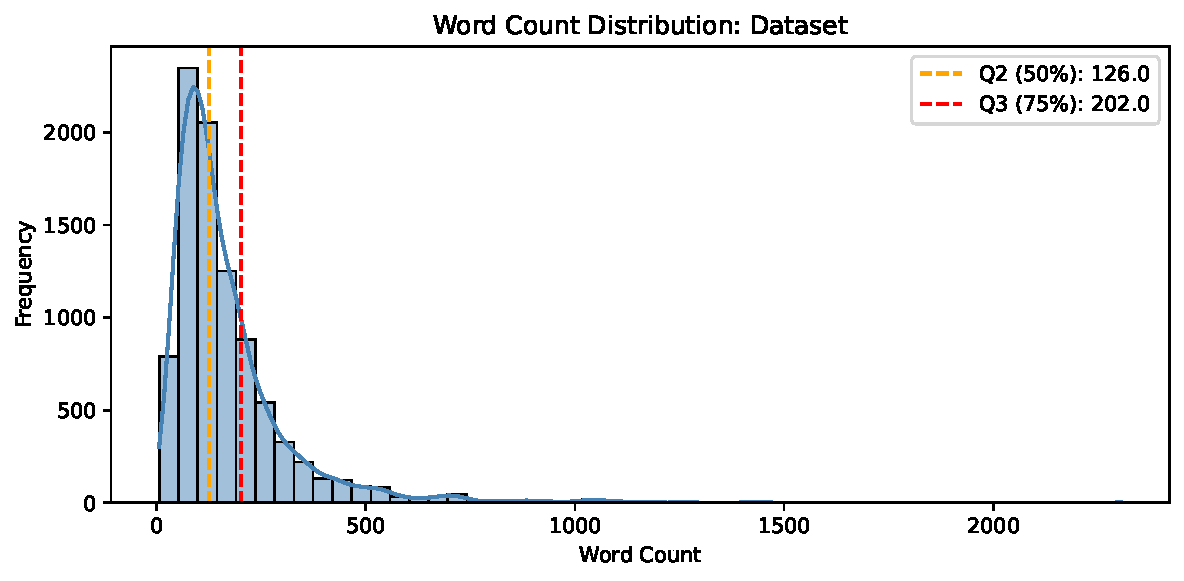
\includegraphics[width=\textwidth]{figures/feedbackqa_word_count.pdf}
        \caption{FeedbackQA: combined word counts (Question + Answer).}
        \label{fig:feedbackqa_word_count}
    \end{subfigure}

    \vspace{0.5em}

    \begin{subfigure}{0.82\textwidth}
        \centering
        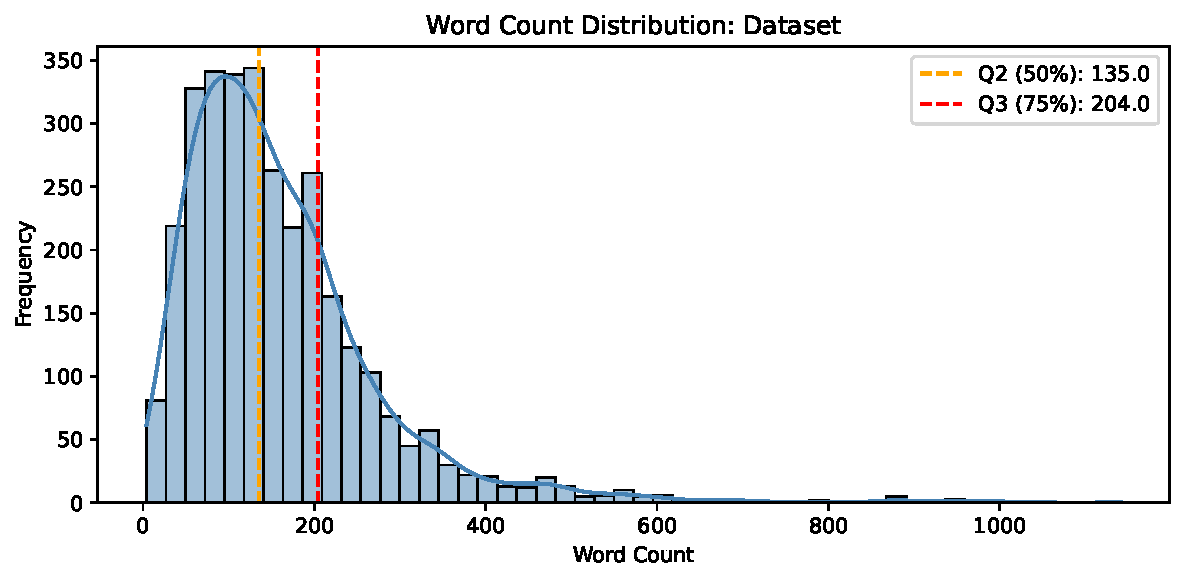
\includegraphics[width=\textwidth]{figures/barter_word_count.pdf}
        \caption{Barter Deals: combined word counts (Title + Body + Requirements).}
        \label{fig:barter_word_count}
    \end{subfigure}

    \caption{Empirical word-count distributions used for the residual verbosity-sensitivity diagnostic. Dashed lines indicate the median and 75th percentile, which define the mature text brackets $D_{Q3}$ and $D_{Q4}$. For FeedbackQA, $Q(0.50)=126$ and $Q(0.75)=202$; for Barter Deals, $Q(0.50)=135$ and $Q(0.75)=204$.}
    \label{fig:word_count_distributions}
\end{figure}



\begin{table}[h]
    \centering
    \caption{Text-length statistics for Barter Deal text sections}
    \label{tab:barter_text_length_stats}
    \begin{tabular}{lrrrr}
    \toprule
    Text Section & Mean Word Count & SD & Median (Q2) & 75th Percentile (Q3) \\
    \midrule
    Body & 81.89 & 72.13 & 64 & 104 \\
    Requirements & 74.92 & 79.55 & 53 & 98 \\
    \bottomrule
    \end{tabular}
\end{table}




\subsection{Rating-Target Distributions}\label{app:rating_distributions}


This subsection reports the full criterion-level EV rating distributions used to support the aggregate rating-regime diagnostics in the main text.

\FloatBarrier

\begin{sidewaysfigure}[p]
    \centering
    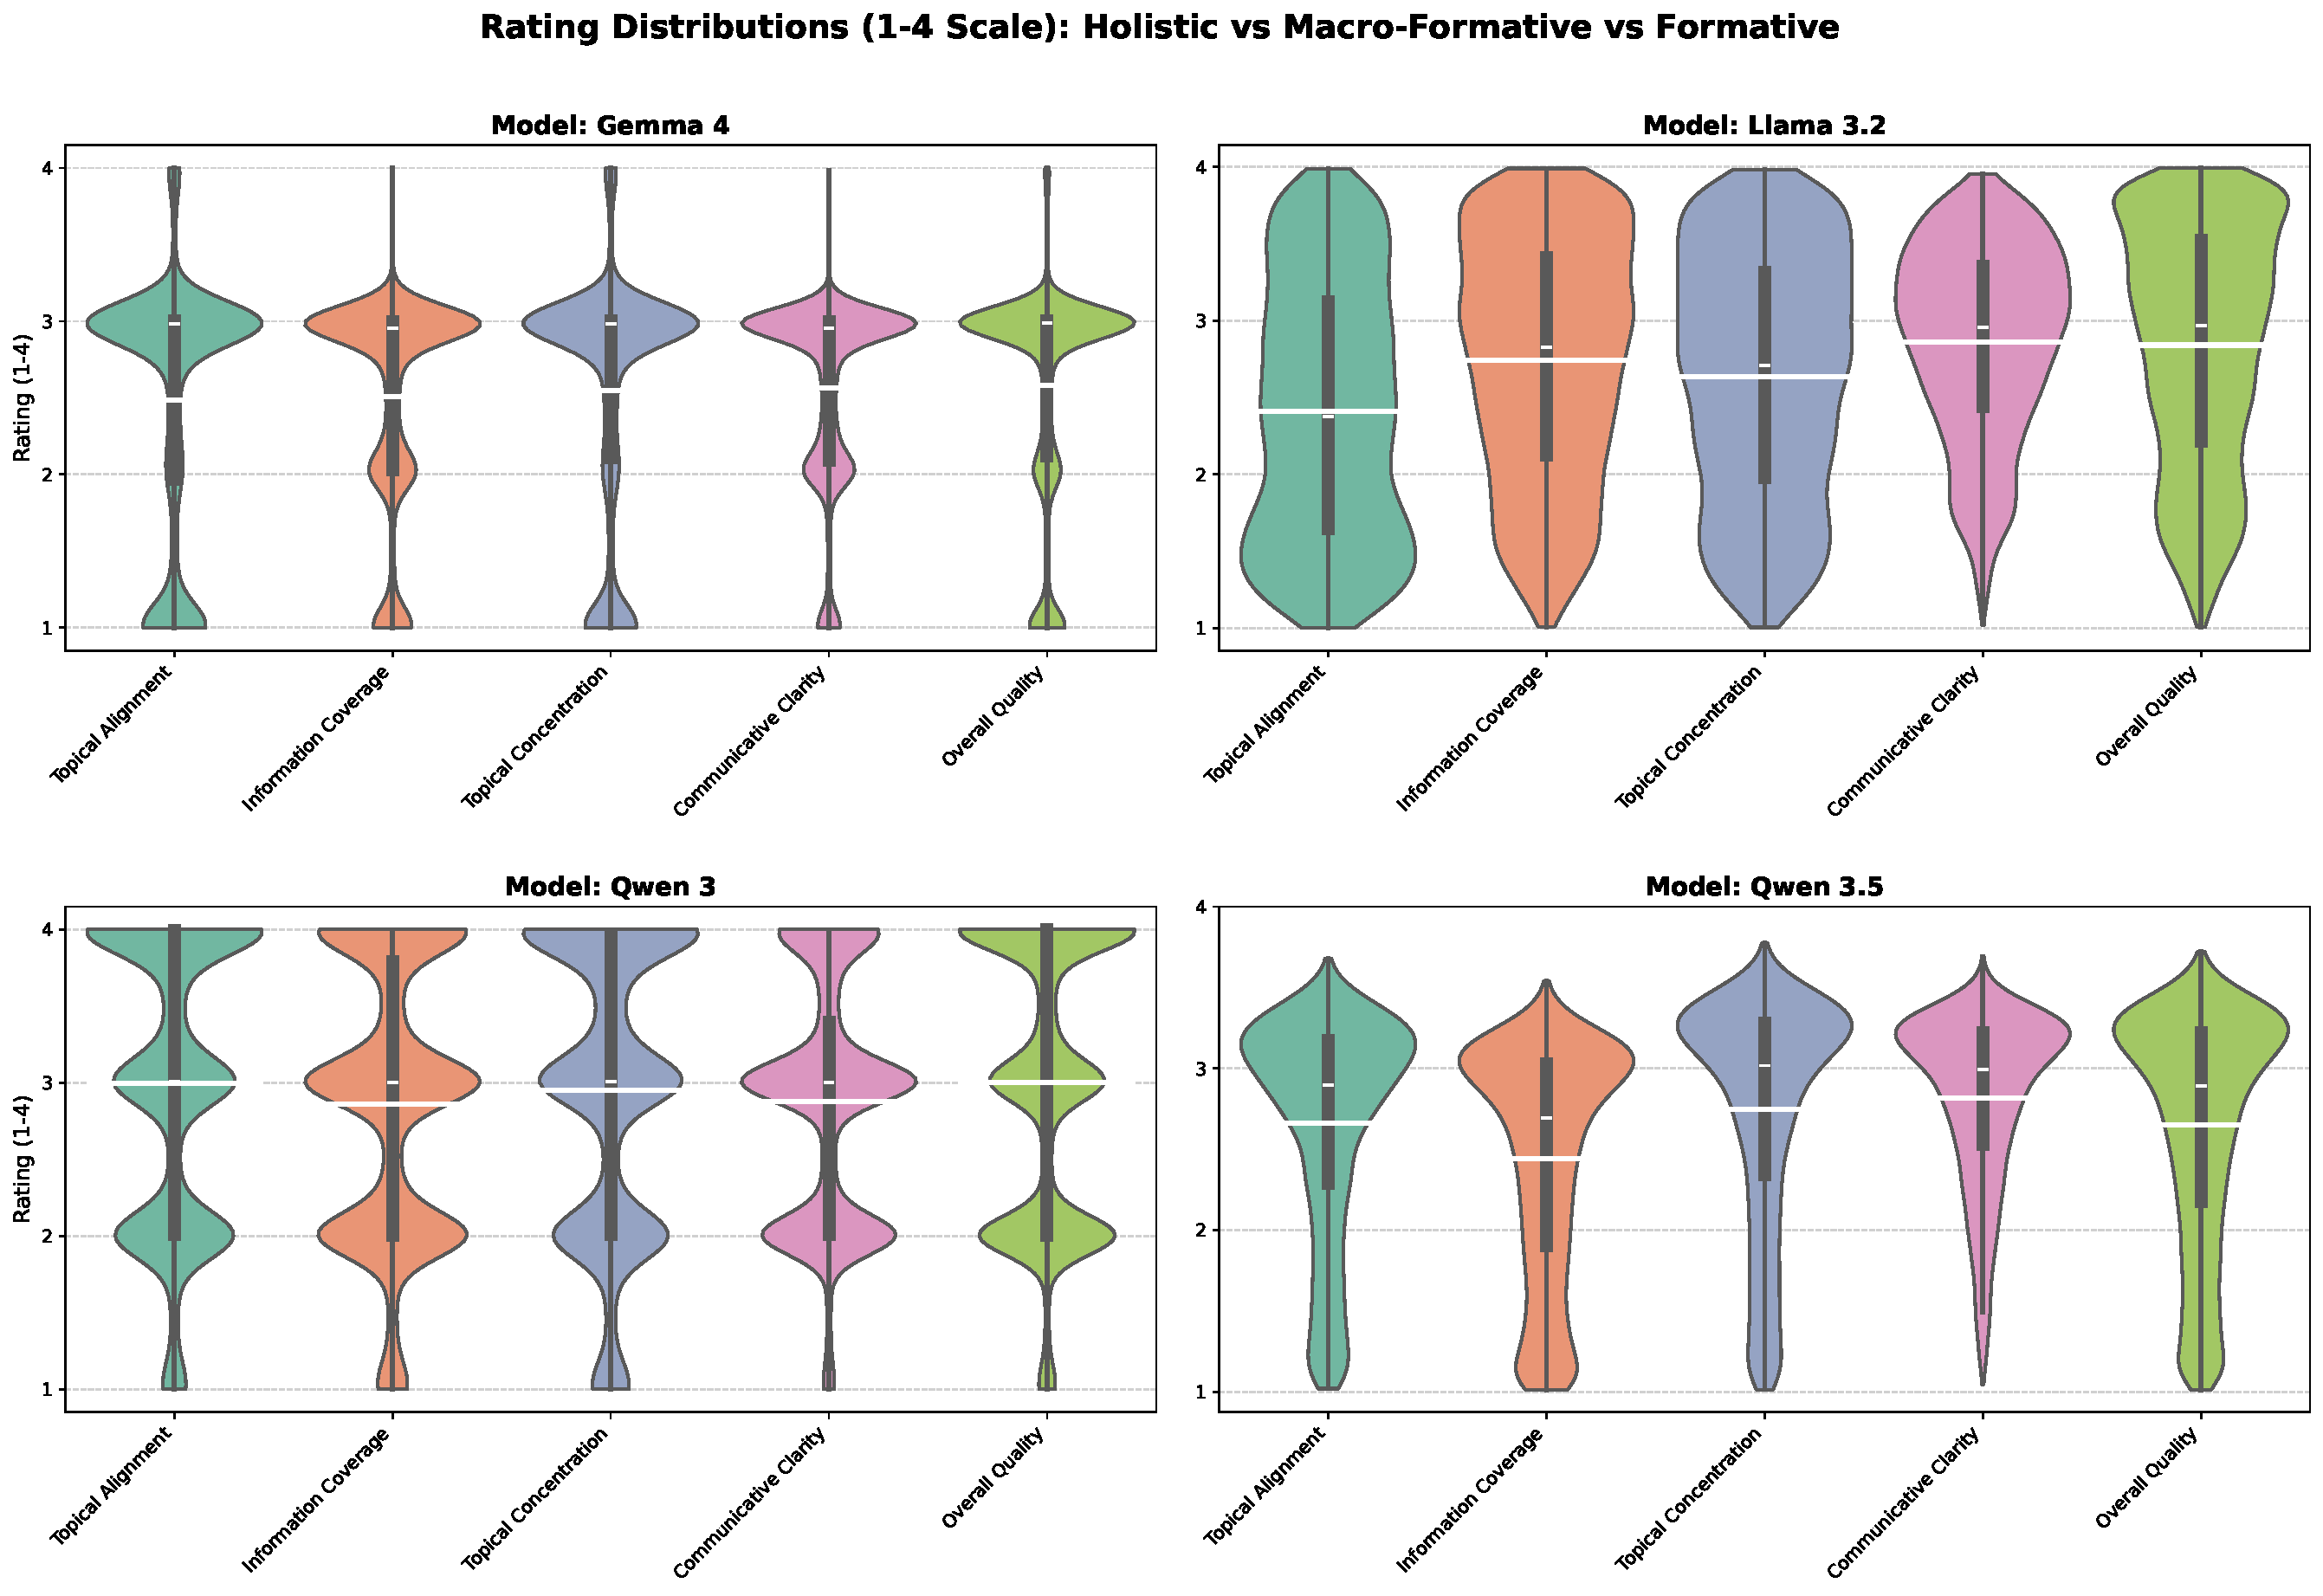
\includegraphics[width=\textwidth]{figures/feedbackqa_rating_distributions.pdf}
    \caption{Rating-target expected-value rating distributions for FeedbackQA.}
    \label{fig:feedbackqa_rating_distributions}
\end{sidewaysfigure}


\begin{sidewaysfigure}[p]
    \centering
    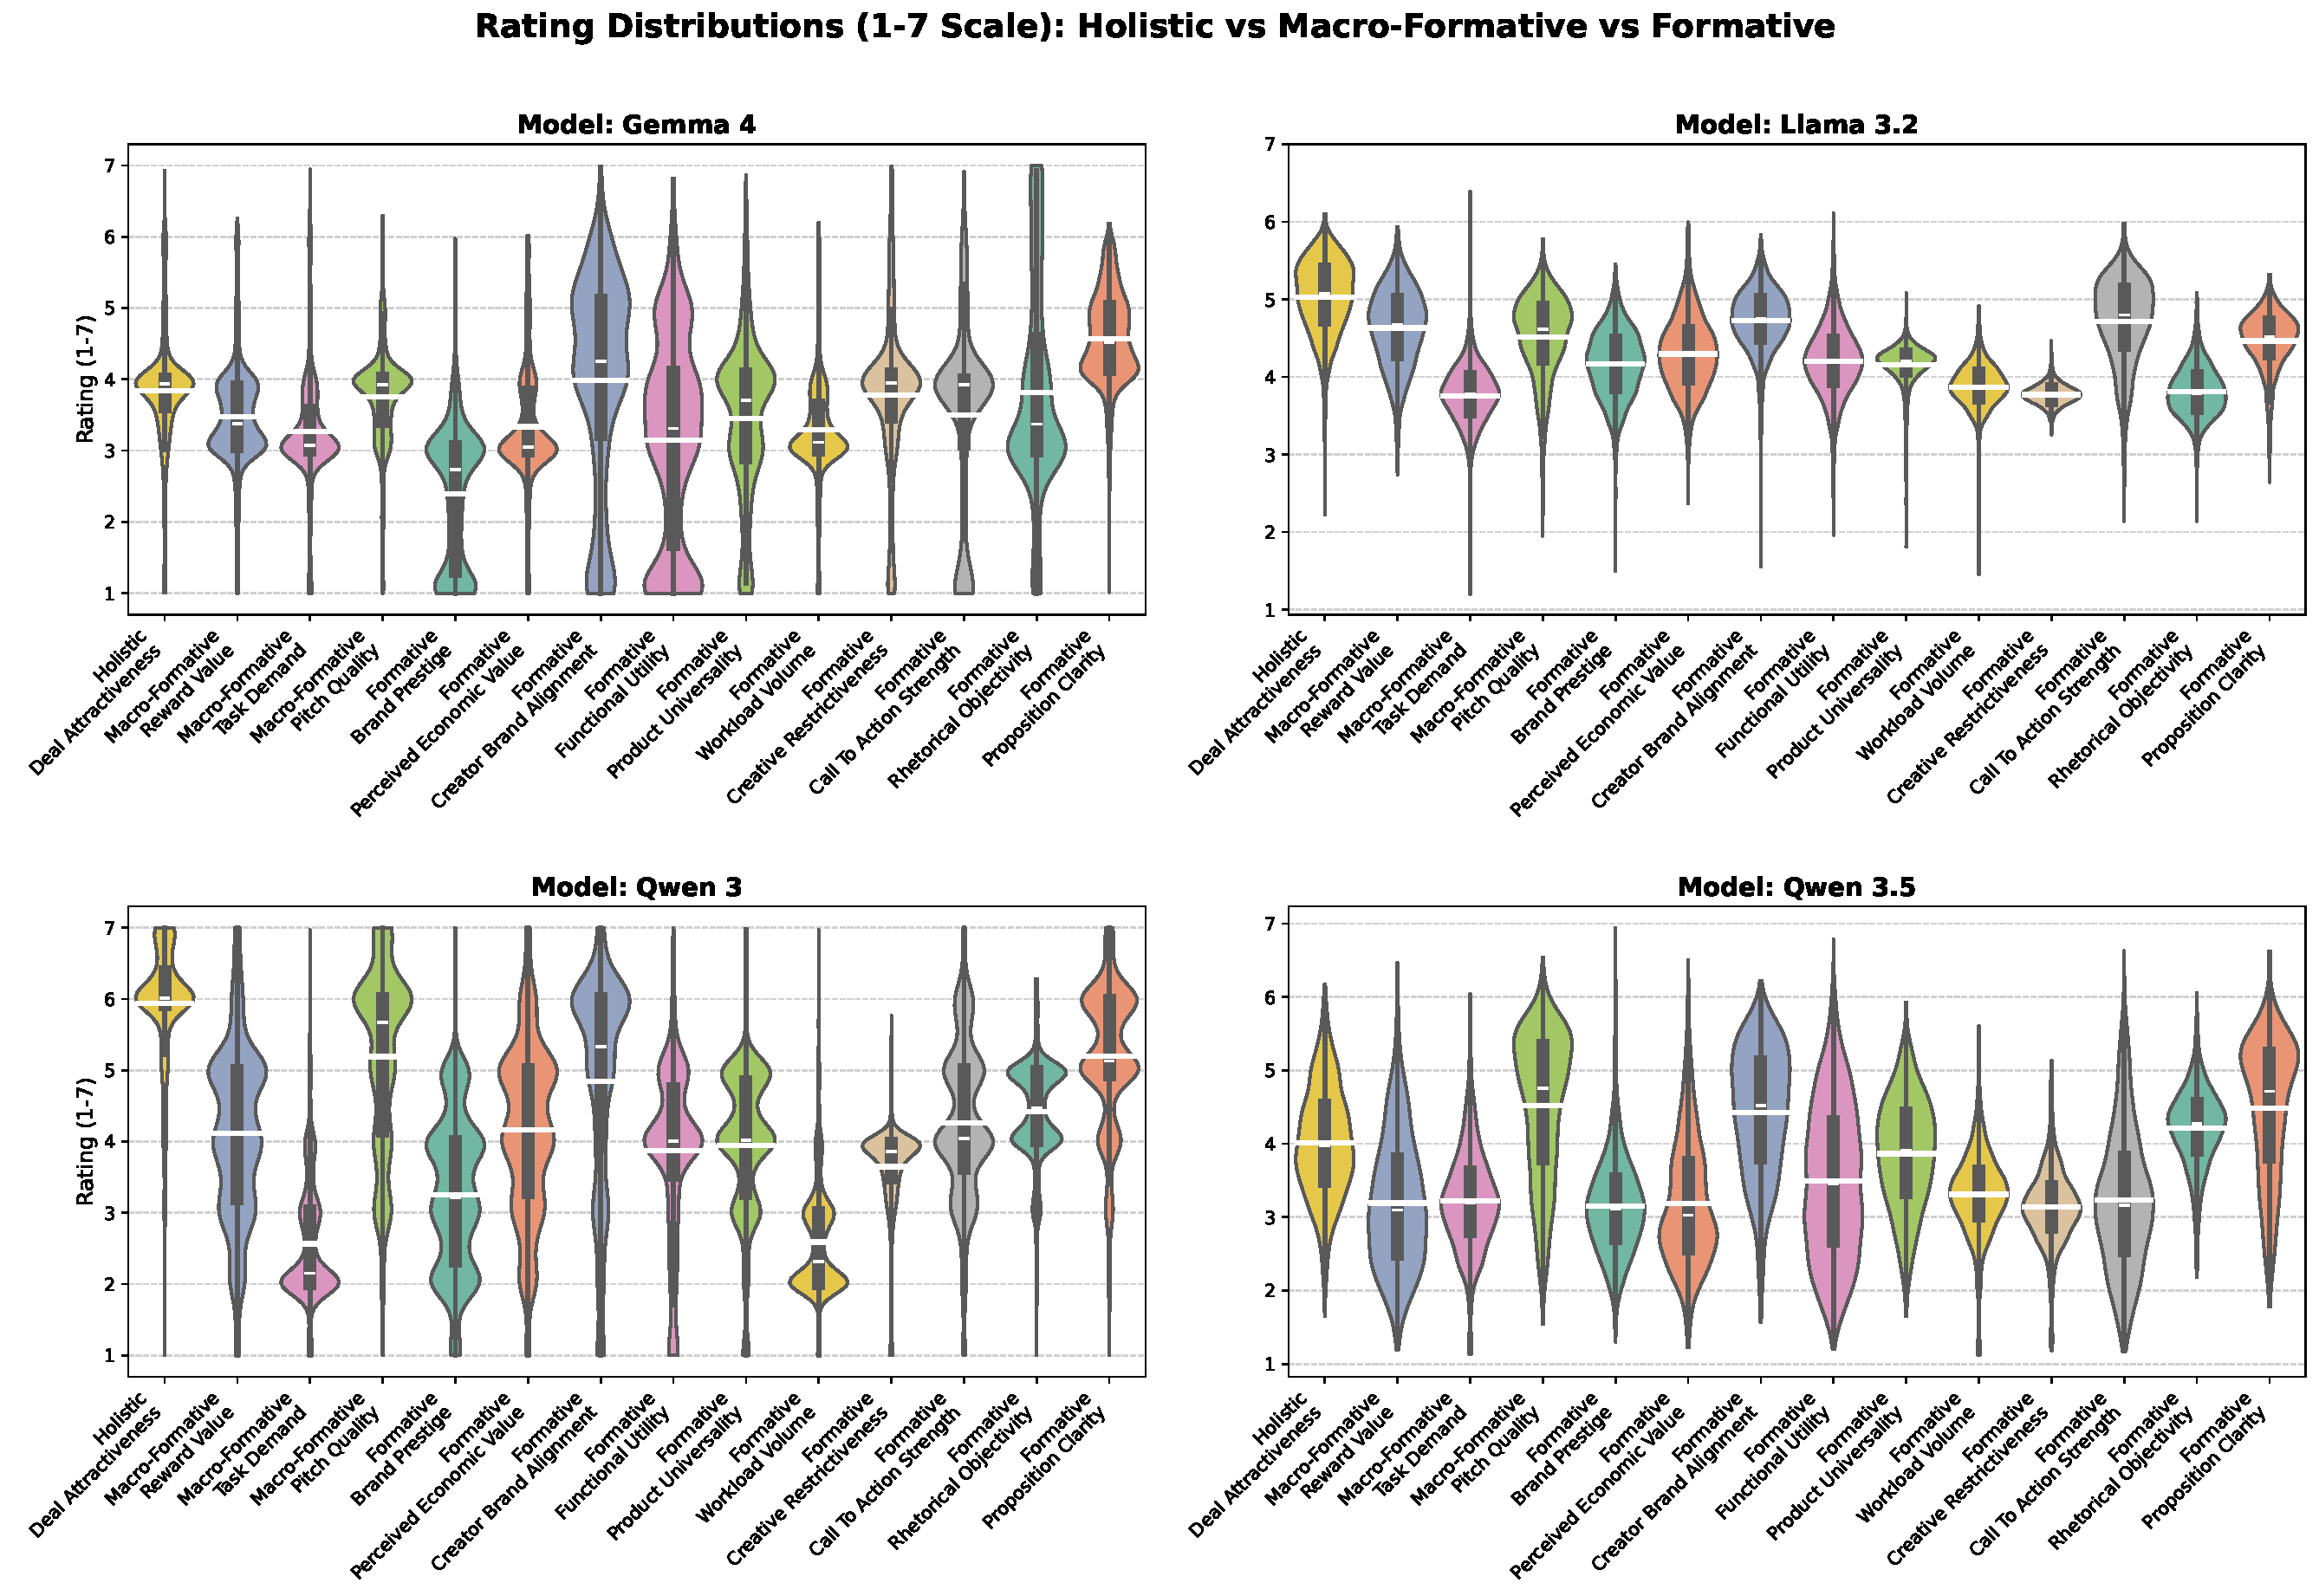
\includegraphics[width=\textwidth]{figures/barter_rating_distributions.pdf}
    \caption{Rating-target expected-value rating distributions for Barter Deals.}
    \label{fig:barter_rating_distributions}
\end{sidewaysfigure}


\FloatBarrier


\subsection{Additional Multicollinearity Diagnostics}\label{app:vif_diagnostics}

\begin{table}
    \caption{VIF Diagnostics for Barter Deals Formative Specifications}
    \label{tab:VIF_barter}
    \begin{tabular}{lccrrl}
    \toprule
    Group & Max VIF & Mean VIF & N VIF > 5 & N VIF > 10 & Multicollinearity \\
    \midrule
    Gemma 4 Formative & 1.79 & 1.36 & 0 & 0 & Limited \\
    Gemma 4 Macro-Formative & 1.70 & 1.49 & 0 & 0 & Limited \\
    Llama 3.2 Formative & 3.70 & 2.54 & 0 & 0 & Limited \\
    Llama 3.2 Macro-Formative & 4.20 & 2.99 & 0 & 0 & Limited \\
    Qwen 3 Formative & 1.97 & 1.49 & 0 & 0 & Limited \\
    Qwen 3 Macro-Formative & 1.34 & 1.25 & 0 & 0 & Limited \\
    Qwen 3.5 Formative & 2.07 & 1.58 & 0 & 0 & Limited \\
    Qwen 3.5 Macro-Formative & 1.34 & 1.26 & 0 & 0 & Limited \\
    \bottomrule
    \end{tabular}

    \begin{flushleft}
    \footnotesize
    \textit{Note.} VIF values are only computed for the LLM-derived evaluations for the Formative and Macro-Formative conditions, and do not include the non-LLM control variables. Values above 5 are interpreted as moderate multicollinearity and values above 10 as substantial multicollinearity.
    \end{flushleft}
\end{table}


\begin{table}
\centering
\caption{VIF Diagnostics for Barter Deals Baseline Control Specification}
\label{tab:VIF_barter_controls}
\begin{tabular}{lccrrl}
\toprule
Specification & Max VIF & Mean VIF & $N_{\mathrm{VIF}>5}$ & $N_{\mathrm{VIF}>10}$ & Multicollinearity \\
\midrule
Baseline Controls & 5.09 & 2.04 & 1 & 0 & Moderate \\
\bottomrule
\end{tabular}

\begin{flushleft}
\footnotesize
\textit{Note.} VIF values are computed for the non-LLM control specification used in the Barter Deals predictive-validity models. The only predictor exceeding 5 is \textit{macro\_category\_Home Cooking \& CPG} with a VIF of $5.09$. No predictor exceeds 10.
\end{flushleft}
\end{table}






